\chapter{Ajout de deux boutons poussoirs}

\section{Montage des boutons}
Comme vous pouvez le voir sur la figure \ref{montageBoutons} nous avons montés les boutons en montage Pull-Down ainsi que évoqué sur la figure \ref{montagePullDown} sur les entrées 8 et 9 de l'Arduino.
\begin{figure}[h]
	\centering
	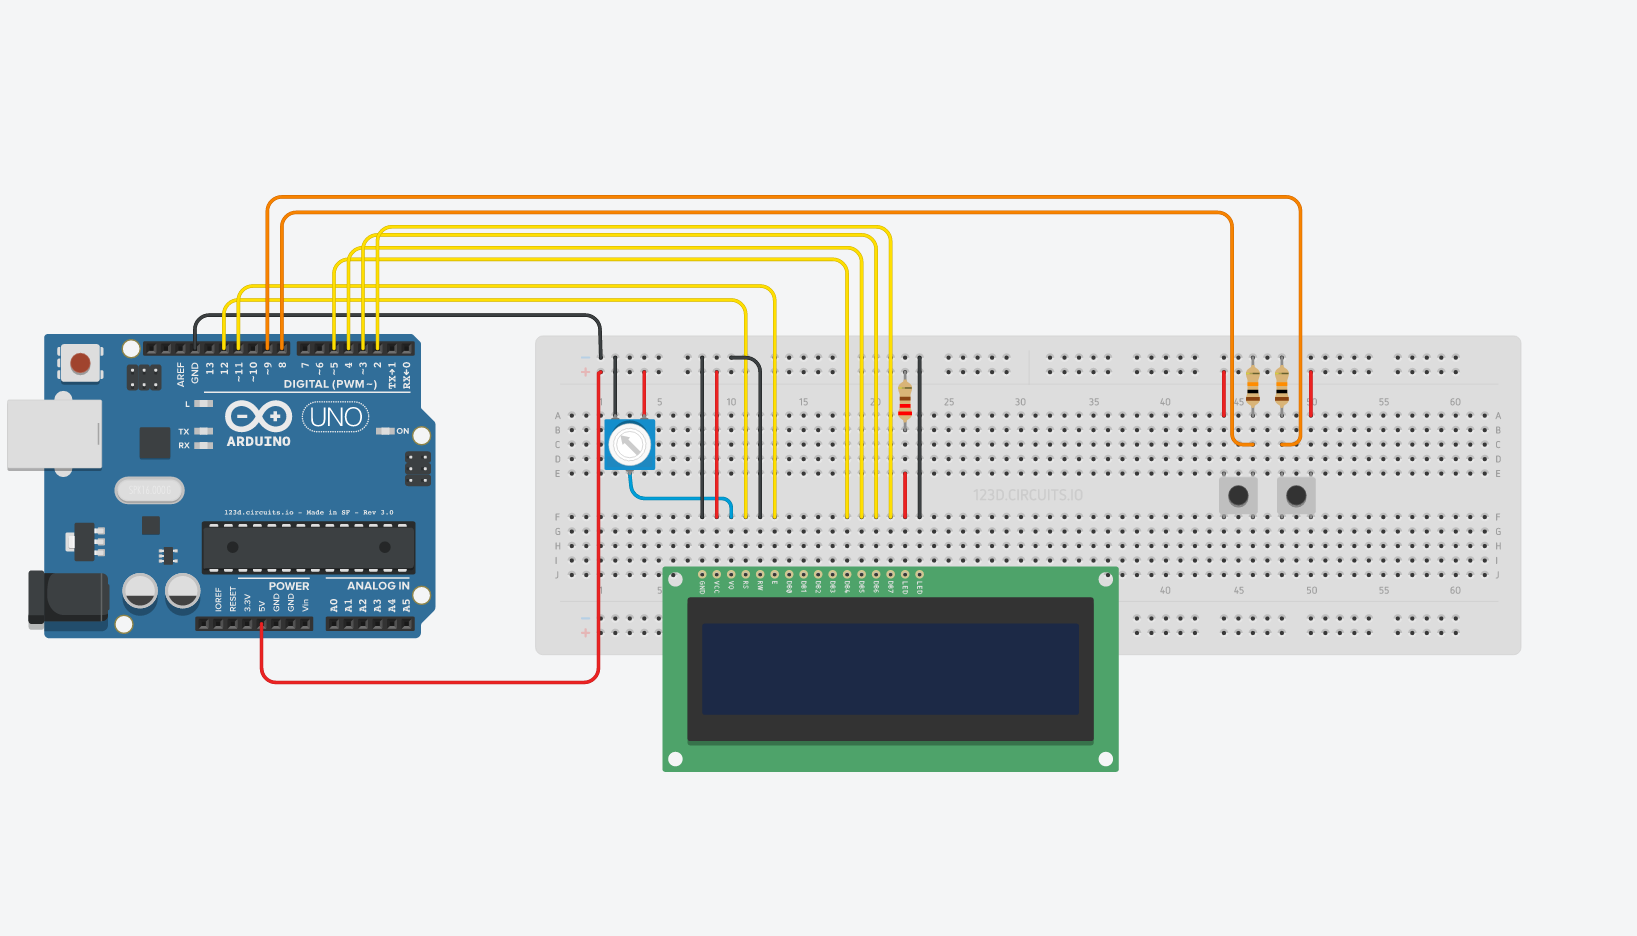
\includegraphics[width=\linewidth]{montageBouttons.png}
    \caption{Montage Boutons}
    \label{montageBoutons}    
\end{figure}

\newpage
\section{Montage Pull-Down}
\paragraph{}
	Nous pouvons remarquer sur le montage de la figure \ref{montageBoutons} deux résistance placées a la sortie des boutons poussoir. Il s'agit de résistance dites "Pull-Down". Ces resistance ont deux roles tres important, elles servent à assurer le bon fonctionnement du bouton, mais également la sécurité du circuit.
    
\begin{figure}[h]
	\centering
	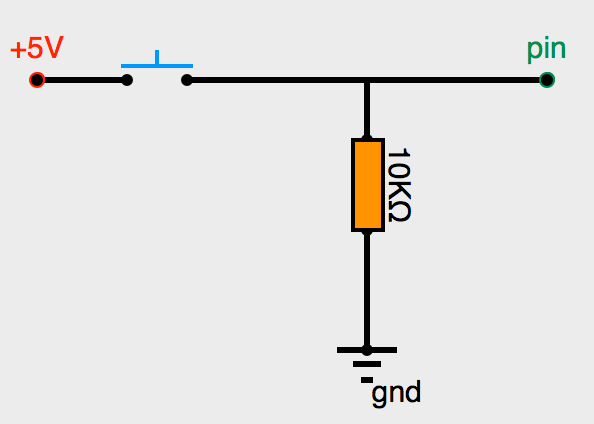
\includegraphics[width=10cm]{boutonPullDown.png}
    \caption{Montage d'une résistance en Pull-Down}
    \label{montagePullDown}
\end{figure}

\paragraph{}
	L'électricité choisis toujours le chemin le moins résistif. Mais si elle n'a pas le choix, elle passe tout de même là où ça résiste.

	Nous allons donc ajouter une résistance à notre circuit. Une assez forte pour que le courant ne passe que s'il y est obligé (ici de $10k\Omega$).
	Si le poussoir est baissé, le courant va du +5V a la pin de l'Arduino. Il ne prendra pas le chemin de la masse car la résistance lui demande un effort(Et dans le cas contraire la resistance protegera le montage d'un court-circuit). La pin de l'Arduino recevra du +5V et indiquera HIGH (ou 1).

	Si le poussoir est levé, donc le circuit ouvert, le très faible courant résiduel qui sortira du pin de l'Arduino sera absorbé par la masse, le pin sera donc bien en LOW (ou 0)



\newpage
\section{Programme}
\underline{Programme utilisé pour tester le bon fonctionnement de l'acquisition des boutons:}
\lstinputlisting[language=c]{Sources/testBoutons.ino}

\newpage
\paragraph{}
\underline{Voici les affichages obtenus:}
\begin{itemize}
	\item Lorsqu'on appuie sur aucun boutons:
    \begin{figure}[h]
    	\centering
        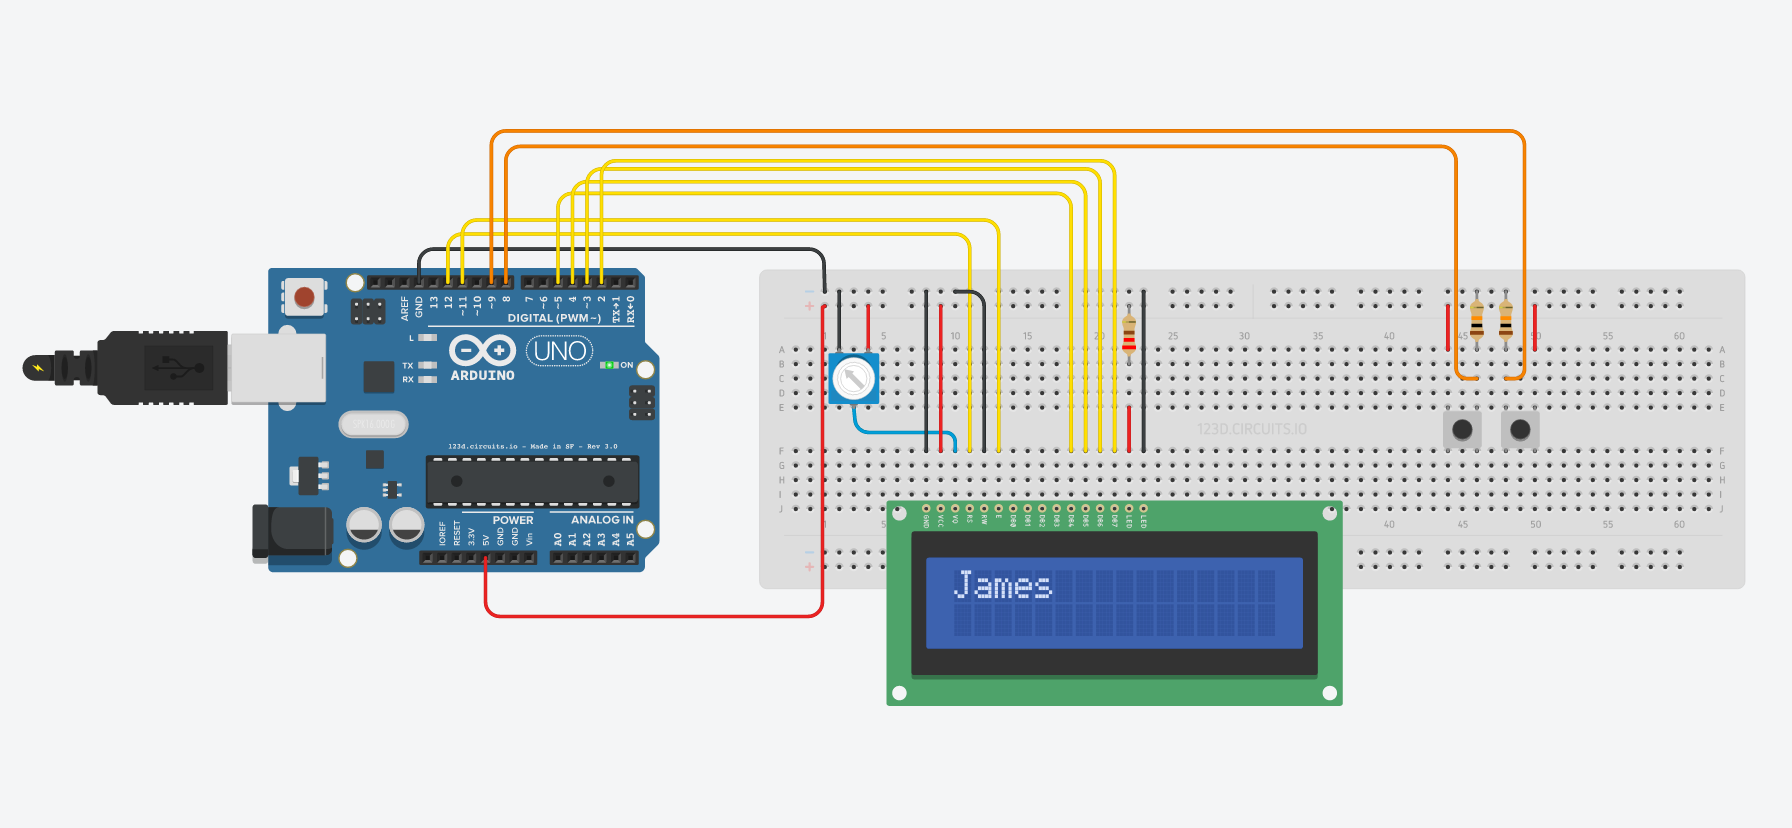
\includegraphics[width=\linewidth]{testbutons_0.png}
        \caption{Test sans appuyer sur les boutons}
        \label{testbutons0}
    \end{figure}
    
    \item Lorsqu'on appuie sur un des 2 boutons:
    \begin{figure}[h]
    	\centering
        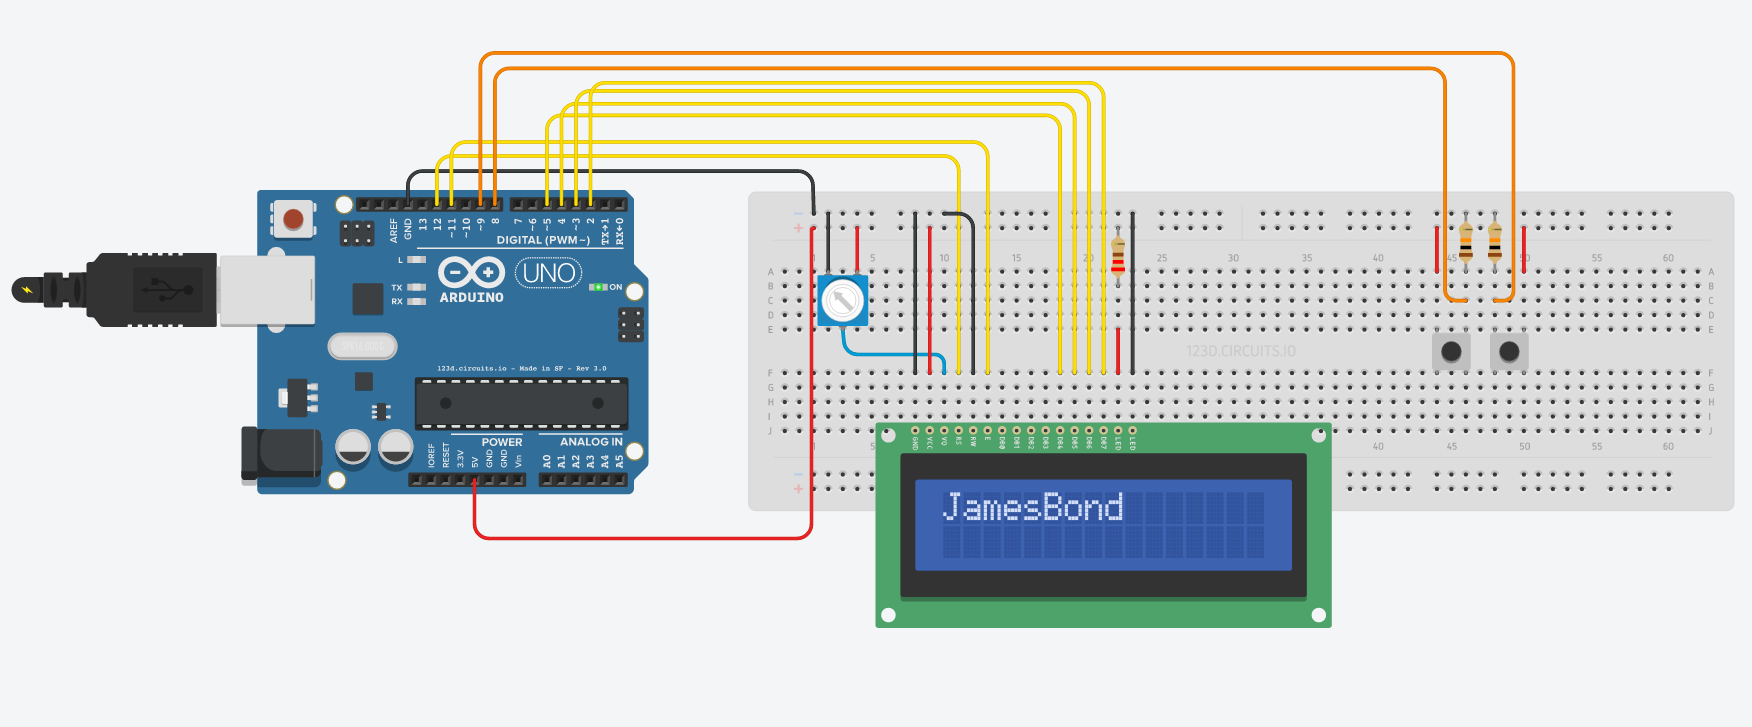
\includegraphics[width=\linewidth]{testbutons_1.png}
        \caption{Test en appuyant sur un des deux boutons}
        \label{testbutons1}
    \end{figure}
\end{itemize}

